% Created 2017-03-24 Sex 14:56
% Intended LaTeX compiler: pdflatex
\documentclass{report}
               \pagestyle{fancy}
\usepackage[utf8]{inputenc}
\usepackage[T1]{fontenc}
\usepackage{graphicx}
\usepackage{grffile}
\usepackage{longtable}
\usepackage{wrapfig}
\usepackage{rotating}
\usepackage[normalem]{ulem}
\usepackage{amsmath}
\usepackage{textcomp}
\usepackage{amssymb}
\usepackage{capt-of}
\usepackage{hyperref}
\usepackage{paralist}
\usepackage{tcolorbox}
\usepackage[table]{xcolor}
\usepackage{lipsum}
\usepackage{caption}
\usepackage{tabu}
\usepackage[subpreambles=true]{standalone}
\usepackage{import}
\usepackage{setspace}
\usepackage{graphics}
\usepackage[linktocpage=true]{hyperref}
\usepackage{tocloft}
\usepackage{minitoc}
\usepackage[portuguese, english]{babel}
\usepackage[utf8]{inputenc}
\date{}
\title{}
\hypersetup{
 pdfauthor={user},
 pdftitle={},
 pdfkeywords={},
 pdfsubject={},
 pdfcreator={Emacs 25.1.1 (Org mode 9.0.5)},
 pdflang={English}}
\begin{document}

\thispagestyle{firststyle}
\IssueTitle{Market Discipline or a Fallout}
\NewsAuthor{Mauricio Rosal, \small\it Chief Economist, PhD}
\NewsEmail{joao.rosal@bgcpartners.com}
\JournalIssue

    \begin{tcolorbox}[colbak=red!5!white, colframe=red!0!white]
      \NewsItem{Market Discipline or a Fallout?}
      \begin{compactitem}
      \item \textit{We understand the balance of risks have changed, unfortunatley, not for the better.}
      \item \textit{A muddling through type of social security reform is becoming more likely as opposed to a material one.}
      \item \textit{This implies a two-fold path going foward: a) market discipline forces a meaningful reform, or b) political forebearnace leads to negative re-pricing for the longer term.}
      \end{compactitem}
    \end{tcolorbox}
\vspace{-0.5cm}

\section{The Two-fold paths}
\label{sec:org10a1df2}
\begin{compactitem}[$\diamond$]
\item \textbf{Balance of risks have changed}. The latest flow of news have
confirmed the difficulties of Mr. Temer to approve the social
secutiry reform as is. While some type of compromising have been
expected from the outset, we believe the latest announcement to
leave State civil servants out of the reform has opened a pandora
box, making it is difficult to predict what is going to come out of
it.

More specifically, once one makes such a type of compromising
involving specific classes of workers, the incentives in place are
such that other classes should soon start to lobby for
favoritism. In addition, there is also the interest of less
organized citizens, such as those leaving off social benefits in
many corners of the country, who hold great voting
relevance. Thence, once sums all that up, the budget of acceptable
concessions from the fiscal adjustment standpoint may start to fall
short of the mounting pressures.
\end{compactitem}

\begin{figure}[h]\centering
\subfloat[#]{
\label{fig:spreads}
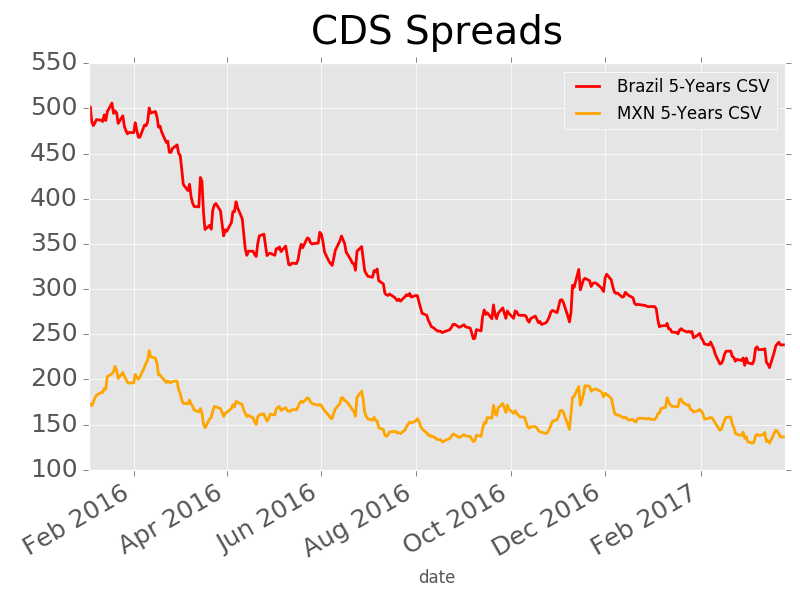
\includegraphics[width=6.5cm]{./images/csv.png}

}
\subfloat[#]{
\label{fig:vix}
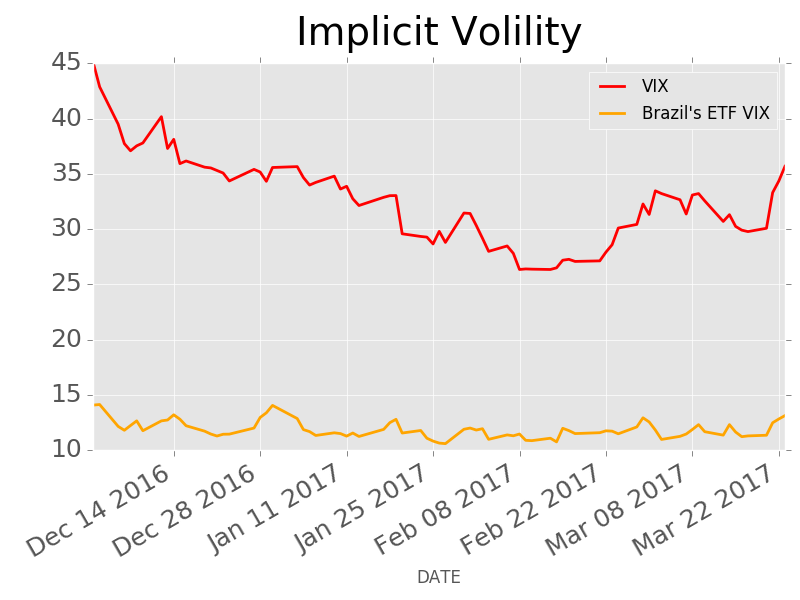
\includegraphics[width=6.5cm]{./images/vix.png}
}

\end{figure}

\begin{itemize}
\item \textbf{A two-fold path}. In light of the fore mentioned, the easy path
towards a reform that comprises a) increases the minimum retirement
age to 65 for both genders; b) ends with retirement of period of
contribution of the system; and c) encompasses rural, urban, private
and public workers alike is no longer possible. In fact, in order to
reach a compromise that contemplates parts of either of these
topics, there ought to be pressure in the opposite direction, and
the only possible candidate to looks in the positions to do so is
the market.

In fact, Brazilian credit spreads as in \ref{fig:spreads}, it's been
standing about 90bps above Mexico's year-to-date, a country holding
a sovereign credit rating about 4 notches above Brazil's. No doubt,
it entails a rather benign vision towards the country's outlook, in
particular, with respect to the country social security system.
Hence, should this perception changes significantly, there is plenty
of room for things to turn sour. In fact, the recent moves
concerning the social security reform have been shrugged off by the
market, and the volatility of Brazilian assets have clearly take off
way from the US's benchmark.

Hence, the question: will the political class remain oblivious to
that and follow their own agenda, or will the kneel to market
pressures? We thinks latter of the most likely candidate, but with
2018 general elections take over their agenda, one should not
dismiss the former altogether.
\end{itemize}



\newpage




\section{Forecastsn}
\label{sec:org01e9a42}


\rowcolors{2}{grey!15}{white}
\begin{center}
\begin{tabular}{lrrr}
\hline
\textbf{Variable} & \textbf{2016} & \textbf{2017E} & \textbf{2018E}\\
\hline
\hline
GDP (yoy \%) & -3.5 & 0.3 & 2.5\\
Selic Rate (\%) & 13.25 & 8.00 & 7.5\\
Fx Rate (BRL per USD) & 3.20 & 3.25 & 3.30\\
CPI (yoy \%) & 6.3 & 4.0 & 4.4\\
Gross Debt to GDP (\%) & 73.0 & 77.2 & 83.2\\
Primary Surplus (\% GDP) & -2.1 & -2.0 & -1.0\\
Trade Balance (\% GDP) & 2.0 & 1.5 & 1.5\\
Current Account (\%GDP) & -1.2 & -1.5 & -2.0\\
Foreign Reserves (xUSD Gross Liabilities) & 1.1 & 1.1 & 1.1\\
\hline
\end{tabular}
\end{center}

\newpage


\section{Disclaimer}
\label{sec:orgbeb03e1}
\url{http://www.bgcpartners.com} \\
\textbf{CONFIDENTIAL:} This document has been sent to you by one of
the BGC entities (collectively BGC) Please see important legal
information and disclaimer relating to this mail at the following
links: \url{http://www.bgcpartners.com/disclaimers/}

Please see for BGC Disclosures. The link contains company and FCA
registration numbers. This e-mail, including its contents and
attachments, if any, are confidential. If you are not the named
recipient please notify the sender and immediately delete it. You may
not disseminate, distribute, or forward this e-mail message or
disclose its contents to anybody else. Copyright and any other
intellectual property rights in its contents are the sole property of
BGC and its affiliates. E-mail transmission cannot be guaranteed to be
secure or error-free.  The sender therefore does not accept liability
for any errors or omissions in the contents of this message which
arise as a result of e-mail transmission.  If verification is required
please request a hard-copy version. Although we routinely screen for
viruses, addressees should check this e-mail and any attachments for
viruses. We make no representation or warranty as to the absence of
viruses in this e-mail or any attachments. Please note that to ensure
regulatory compliance and for the protection of our customers and
business, we may monitor and read e-mails sent to and from our
server(s).  The registered offices of the BGC entities are at 1
Churchill Place, London, E14 5RD.  For any issues arising from this
email please reply to the sender.  The FCA register appears at
\url{http://www.FCA.org.uk/register/}.  The FCA regulates the financial
services industry in the United Kingdom and is located at 25 The North
Colonnade, Canary Wharf, London, E14 5HS.  BGC Financial LP CFTC Rule
1.55(K) Firm Specific Disclosure Statement
\end{document}
